\chapter{Exemples}

\section{Programme Matlab}

\begin{lstlisting}
%% Résistance en traction axiale

sigma_trac = P/A; %Pa
delta_p = P*L/(A*E); %m

%% Réaction en effort tranchant

M = P/2*(1+l); %N.m % Moment fléchissant  en l 
sigma_flex = -M*0.5*d_ext/I; % Pa % Contrainte
epsilonn = sigma_flex/E; % m % Déformation
rho = E*I/M; %m M % rayon de courbure

%% Dilatation thermique

delta_t_max = alpha*L*(temp_max-temp_ref); %microm
delta_t_min = alpha*L*(temp_min-temp_ref); %microm

%% Masse

masse = densite*A*L; %kg

\end{lstlisting}

\section{Tableau simple}

\begin{tabu}{| l | c | c | c | c |}
\hline 
\Xhline{2\arrayrulewidth}
\textbf{Désignation} &
\textbf{Nombre d'heures} &
\textbf{Nombre de personnes} &
\textbf{Total}
\textbf{(40\$/h)}\\ \hline
  Réunion 1 &
  2.5 &
  5 &
   500\\
  Réunion 2 &
  3 &
  5 &
   600\\
  Réunion 3 &
  3 &
  5 &
  600\\
  Réunion 4 &
  6&
  1200 &
   500\\
  Travail individuel &
  60 &
  2 &
   4800\\
   Travail individuel  &
  40 &
  3 &
   4800\\ \hline 
\multicolumn{3}{|c|}{{\textbf{Sous-total
}}} &
 {\textbf{12 500}}\\
\multicolumn{3}{|c|}{{\textbf{TPS
(5\%):}}} &
 {\textbf{625}}\\
\multicolumn{3}{|c|}{{\textbf{TVQ
(9.975\%):}}} &
 {\textbf{1 247}}\\ \hline
\multicolumn{3}{|c|}{{\textbf{Total
: }}} &
 {\textbf{14 372\$}}\\
\hline 
\Xhline{2\arrayrulewidth}
\end{tabu}

\section{Tableau complexe avec légende}

\begin{table}[H] \label{fonctions-principales}
		\noindent \begin{tabu}{ |>{\centering}m{2cm} |>{\centering}m{0.5cm}| >{\centering}m{3cm} |>{\centering}m{0.5cm}| >{\centering}m{3cm} |>{\centering}m{2.5cm} |>{\centering} m{2cm} |}
		\hline 
		\Xhline{2\arrayrulewidth}
		% En-tête
		\textbf{Type} & 
		\textbf{\#} & 
		\textbf{Description} & 
		\textbf{K} & 
		\textbf{Critères} & 
		\textbf{Niveau} & 
		\textbf{Flexibilité} \tabularnewline
		% Ligne 1
		\hline
		\multirow{5}{*}{Usage} & 
		\multirow{5}{*}{1.1} & 
		\multirow{5}{*}{\parbox{3cm}{\centering Déplacer des personnes sur un terrain pentu}} & 
		\multirow{5}{*}{5} &
		Pente moyenne & 
		$25\%$  & 
		$\pm 2\%$ \tabularnewline \cline{5-7}
		% Ligne 2
		 &  
		 &  
		 & 
		 & 
		 Distance & 
		 2558~m & 
		 $\pm 20$ m \tabularnewline \cline{5-7}
		 % Ligne 3
		 &  
		 &  
		 & 
		 & 
		 Temps & 
		 7~min & 
		 $-1$ min \tabularnewline  \cline{5-7}
		 % Ligne 4
		 &  &  & &  
		 Nb. de passagers & 
		 2 & 
		 - \tabularnewline  \cline{5-7}
		 % Ligne 5
		 &  
		 &  
		 & 
		 & 
		 Chargement total & 
		 310~kg & 
		 $\pm 40$ kg \tabularnewline 
		\hline
		% Ligne 6
		\multirow{4}{*}{Sécurité} & 
		\multirow{4}{*}{1.2} & 
		\multirow{4}{*}{\parbox{3cm}{\centering Embarquer et débarquer des personnes dans un délai raisonnable}} &
		\multirow{4}{*}{5} & 
		Temps d'embarquement & 
		15 s & 
		$\pm 5$ s \tabularnewline \cline{5-7}
		% Ligne 7
		 & 
		 & 
		 & 
		 & 
		 Embarquer du matériel & 
		 2 paires de skis & 
		 $\pm 1$ paire\tabularnewline \cline{5-7}
		 %Ligne 8
		 & 
		 &
		  & 
		  & 
		 Différence de hauteur cabine / point d'embarquement & 
		 $0$ cm & 
		 $\pm 2$ cm\tabularnewline \cline{5-7}
		% Ligne 9
		 & 
		 & 
		 & 
		 & 
		 Jeu cabine / point d'embarquement  & 
		 6 cm & 
		 $\pm 1$ cm \tabularnewline
		\hline
		% Ligne 10
		\multirow{3}{*}{Utilisabilité} & 
		\multirow{2}{*}{1.3} & 
		\multirow{2}{*}{\parbox{3cm}{\centering Fluidité du transport}} & 
		\multirow{2}{*}{5} & 
		Débit de personnes à remonter & 
		hiver: 1440 pers./h, été: 720 pers./h et 720 vélos/h & 
		$+ 20$ pers./h $+ 20$ vélos/h\tabularnewline \cline{5-7}
		% Ligne 11
		&
		 & 
		 & 
		 & 
		Rythme d'arrivée des cabines &
		1 cabine toutes les 5 s &
		$\pm 1$ s\tabularnewline  \cline{2-7}
		% Ligne 12
		& 
		1.4 & 
		Contrôle de la vitesse en gare & 
		5 & 
		Vitesse à l'embarquement et au débarquement &
		$3 $ m/s &
		$\pm 1$ m/s \tabularnewline
		\hline
		\Xhline{2\arrayrulewidth} 
		\end{tabu} 
		\caption{Fonctions principales}
		\end{table}
		
\section{Figure avec légende}

	\begin{figure}[H]
	\centering
	\fbox{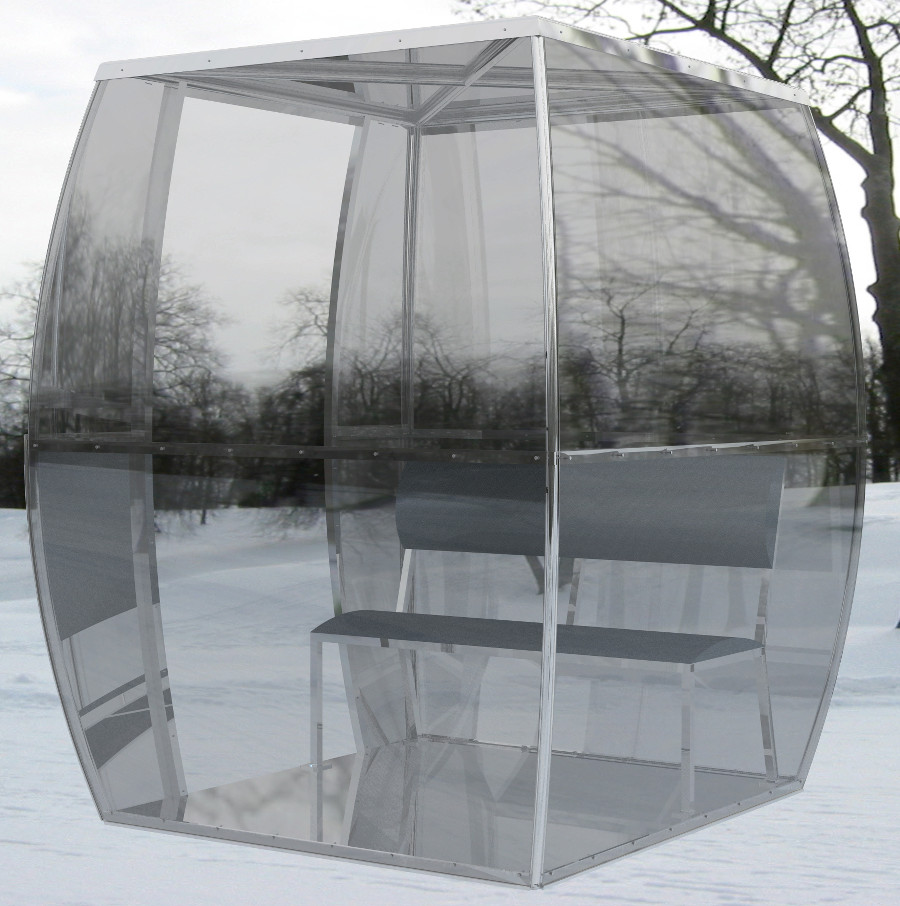
\includegraphics[width=\textwidth-0.5cm]{images/cabine-final-2.jpg}}
	\caption{Vue en perspective de la cabine}
	\end{figure}